\documentclass[main.tex]{subfiles}
\begin{document}
\begingroup

\renewcommand{\cleardoublepage}{}

\renewcommand{\clearpage}{}
	\newpage
	\chapter{Appendix}
		\section{Abbreviations}
		ROS - Robot Operating System \\
		HSR - Human Service Robot \\
		SUTURO - Sudo Tidy Up My Room \\
		NLP - Natural Language Processing \\
		CRAM - Cognitive Robot Abstract Machine \\
		URDF - Universal Robotic Description Format \\
		CAS - Common Analysis Structure\\
		KNN - K Nearest Neighbor\\
		RDF - Resource Description Framework\\
		GUI - General User Interface \\
		LLIF - Low-Level Interfacing \\
		COMF - Common Functions \\
		\section{Communication}
			\subsection{Messages}
			\label{msgs}
				\subsubsection{Object In Gripper}\label{msg_obj_in_gripper}
				\subsubsection{Object In Gripper Info}
				This message is sent, when manipulation grasps or places a object.
				\begin{itemize}
					\item object\_frame\_id - frame id of the object
					\item goal\_pose - new pose of the object if placed
					\item mode - GRASPED or PLACED
				\end{itemize}
					\begin{lstlisting}
uint8 GRASPED=0
uint8 PLACED=1
		
string object_frame_id
geometry_msgs/PoseStamped goal_pose
uint8 mode
\end{lstlisting}
				\subsubsection{Speech Generation}
				\label{msg_speech_generation}
                
                This message is only a could have been, for how Planning could have called the SpeechGeneration node.\\
                The message contains three elements on witch a sentence is build. \textit{Type} describes the task the robot has done. These are: moving/driving to a location, grabbing something, moving a object or placing a object. The information whether the robot says it has done, is doing or will do something is contained in the \textit{Tense}. The \textit{Attributes} contain extra information for the sentence. See \hyperref[msg_speech_generation_attribute]{Speech Generation Attribute}.
                
				
					\begin{lstlisting}
uint8 MOVE=0
uint8 GRABBING=1
uint8 MOVEOBJECT=2
uint8 PLACING=3
		
uint8 FUTURE=50
uint8 PRESENT=51
uint8 PAST=52
		
uint8 Type
		
uint8 Tense
		
SpeechgenerationAttribute[] Attributes
\end{lstlisting}
				\subsubsection{Speech Generation Attribute}
				\label{msg_speech_generation_attribute}
				The Speech Generation Attribute message is used inside the \hyperref[msg_speech_generation]{Speech Generation message}. This message contains one \textit{Type} and one \textit{Content} attribute.\\
                For example the \hyperref[msg_speech_generation]{Speech Generation message} could contain the information the robot is going to move an object. In this case the \textit{Speech Generation Attribute} might contain the information, that the object is a red pringles can. (This would mean type = 0 and Content = "red pringles can"). Alternatively the objectID, used by KnowRob, could be used. When the message contains a surface, the content would be the name of the surface directly. (e.g. "big table")
                
					\begin{lstlisting}
uint8 OBJECTNAME=0
uint8 OBJECTID=1
uint8 STARTSURFACE=2
uint8 GOALSURFACE=3
					
uint8 Type
string Content
\end{lstlisting}
				\subsubsection{Static Command}
				\label{msg_static_command}
				The \textit{Static Command} is send from the \hyperref[textparser]{textparser} node to Planning. It is send when a sentence commanding the robot to start, stop or continue is actions, is recognized.
					\begin{lstlisting}
uint8 START=0
uint8 STOP=1
uint8 CONTINUE=2
		
uint8 command
\end{lstlisting}
				\subsection{Actions}
				\label{actions}
					\subsubsection{Move Base}
					\label{msg_move_base}
						\href{http://wiki.ros.org/move_base_msgs/MoveBaseAction}{ROS Move Base Reference}
					\subsubsection{Extract Object Info}
					\label{msg_extract_object_info}
						This action is sent when the \textit{RoboSherlock} should be triggered and when \textit{RoboSherlock} is done perceiving and returning its results.
					\begin{itemize}
						\item visualize - more visual output from \textit{RoboSherlock}
						\item regions - the regions which should be processed by \textit{RoboSherlock}
						\item detectionData - contains the objects detected by the \textit{RoboSherlock} pipeline
						\item
					\end{itemize}
					\begin{lstlisting}
bool visualize
string[] regions
---
ObjectDetectionData[] detectionData
---
string feedback
\end{lstlisting}
					\subsubsection{Store Object Info}
					\label{msg_store_object_info}
						This action is sent when the data sent by Perception is forwarded to Knowledge.
						\begin{itemize}
						\item detectionData - contains the objects detected by Perception
						\item succeeded - returns, if the objects are correctly stored
						\item feedback - is able to return a feedback about problems regarding the data. It doesn't return anything right now.
						\end{itemize}
						\begin{lstlisting}
#goal definition
suturo_perception_msgs/ObjectDetectionData[] detectionData
---
#result definition
bool succeeded
---
#feedback
string feedback
\end{lstlisting}
					\subsubsection{Take Pose}
					\label{msg_take_pose}
					\subsubsection{Take Pose Info}
						This action is called to move the HSR into a certain pose.
						\begin{itemize}
							\item pose\_mode - determines the pose
							\item gaze\_point - point to look at in GAZE mode
							\item head\_pan\_joint - joint value in FREE mode
							\item head\_tilt\_joint - joint value in FREE mode
							\item arm\_lift\_joint - joint value in FREE mode
							\item arm\_flex\_joint - joint value in FREE mode
							\item arm\_roll\_joint - joint value in FREE mode
							\item wrist\_flex\_joint - joint value in FREE mode
							\item wrist\_roll\_joint - joint value in FREE mode
							\item --------------------------------------------
							\item error\_code - result: SUCCESS or FAILED
							\item --------------------------------------------
							\item torso\_joint\_state - feedback: not implemented
						\end{itemize}
					\begin{lstlisting}
uint8 FREE=0
uint8 NEUTRAL=1
uint8 LOOK_LOW=2
uint8 LOOK_HIGH=3
uint8 LOOK_FLOOR = 4
uint8 GAZE=5
		
uint8 pose_mode
geometry_msgs/Vector3 gaze_point
		
float32 head_pan_joint
float32 head_tilt_joint
float32 arm_lift_joint
float32 arm_flex_joint
float32 arm_roll_joint
float32 wrist_flex_joint
float32 wrist_roll_joint
---
uint8 SUCCESS=0
uint8 FAILED=1
uint8 error_code
---
float64 torso_joint_state
\end{lstlisting}
				\subsubsection{Move Gripper}
				\label{msg_move_gripper}
				\subsubsection{Move Gripper Info}
				This action is called to move the gripper of the HSR into a certain pose.
				\begin{itemize}
					\item goal\_pose - target pose for the gripper
					\item --------------------------------------------
					\item error\_code - result: SUCCESS or FAILED
					\item --------------------------------------------
					\item tf\_gripper\_to\_goal - feedback: not implemented
				\end{itemize}
					\begin{lstlisting}
geometry_msgs/PoseStamped goal_pose
---
uint8 SUCCESS = 0
uint8 FAILED = 1
uint8 error_code
---
geometry_msgs/TransformStamped tf_gripper_to_goal #goal frame
\end{lstlisting}
				\subsubsection{Grasp}
				\label{msg_grasp}
				\subsubsection{Grasp Info}
				This action is called to grasp an object.
				\begin{itemize}
					\item object\_frame\_id - name of the object
					\item goal\_pose - target pose for the gripper to grasp
					\item object\_size - size of the object
					\item grasp\_mode - grasp object from FRONT, TOP or FREE (orientation of gripper defined in pose)
					\item --------------------------------------------
					\item error\_code - result: SUCCESS or FAILED
					\item --------------------------------------------
					\item tf\_gripper\_to\_goal - feedback: not implemented
					\item gripper\_joint\_state - feedback not implemented
				\end{itemize}
					\begin{lstlisting}
uint8 FREE=0
uint8 FRONT=1
uint8 TOP=2
		
string object_frame_id
geometry_msgs/PoseStamped goal_pose 
geometry_msgs/Vector3 object_size
uint8 grasp_mode
---
uint8 SUCCESS=0
uint8 FAILED=1
		
uint8 error_code
---
geometry_msgs/TransformStamped tf_gripper_to_object
float64 gripper_joint_state\end{lstlisting}
				\subsubsection{Place}
				\label{msg_place}
				\subsubsection{Place Info}
				This action is called to place an object.
				\begin{itemize}
					\item object\_frame\_id - name of the object
					\item goal\_pose - target pose for the object
					\item place\_mode - grasp object from FRONT, TOP or FREE (orientation of gripper defined in pose)
					\item --------------------------------------------
					\item error\_code - result: SUCCESS or FAILED
					\item --------------------------------------------
					\item tf\_gripper\_to\_goal - feedback: not implemented
					\item gripper\_joint\_state - feedback not implemented
				\end{itemize}
					\begin{lstlisting}
uint8 FREE=0
uint8 FRONT=1
uint8 TOP=2
		
string object_frame_id
geometry_msgs/PoseStamped goal_pose
uint8 place_mode
---
uint8 SUCCESS=0
uint8 FAILED=1
uint8 error_code
---
geometry_msgs/TransformStamped tf_object_to_goal
float64 gripper_joint_state
\end{lstlisting}
				\subsubsection{Store Object Info}
				\label{msg_store_object_info}
				\begin{itemize}
					\item detectionData - contains the objects found by the \textit{RoboSherlock} pipeline, already filtered for useful objects
					\item succeed - was the action successfull or not
					\item feedback - feedback of the action 
				\end{itemize}
					\begin{lstlisting}
suturo_perception_msgs/ObjectDetectionData[] detectionData
---
bool succeeded
---
string feedback
\end{lstlisting}
		\section{Diagrams}
		\begin{figure}[H]
			\centering
			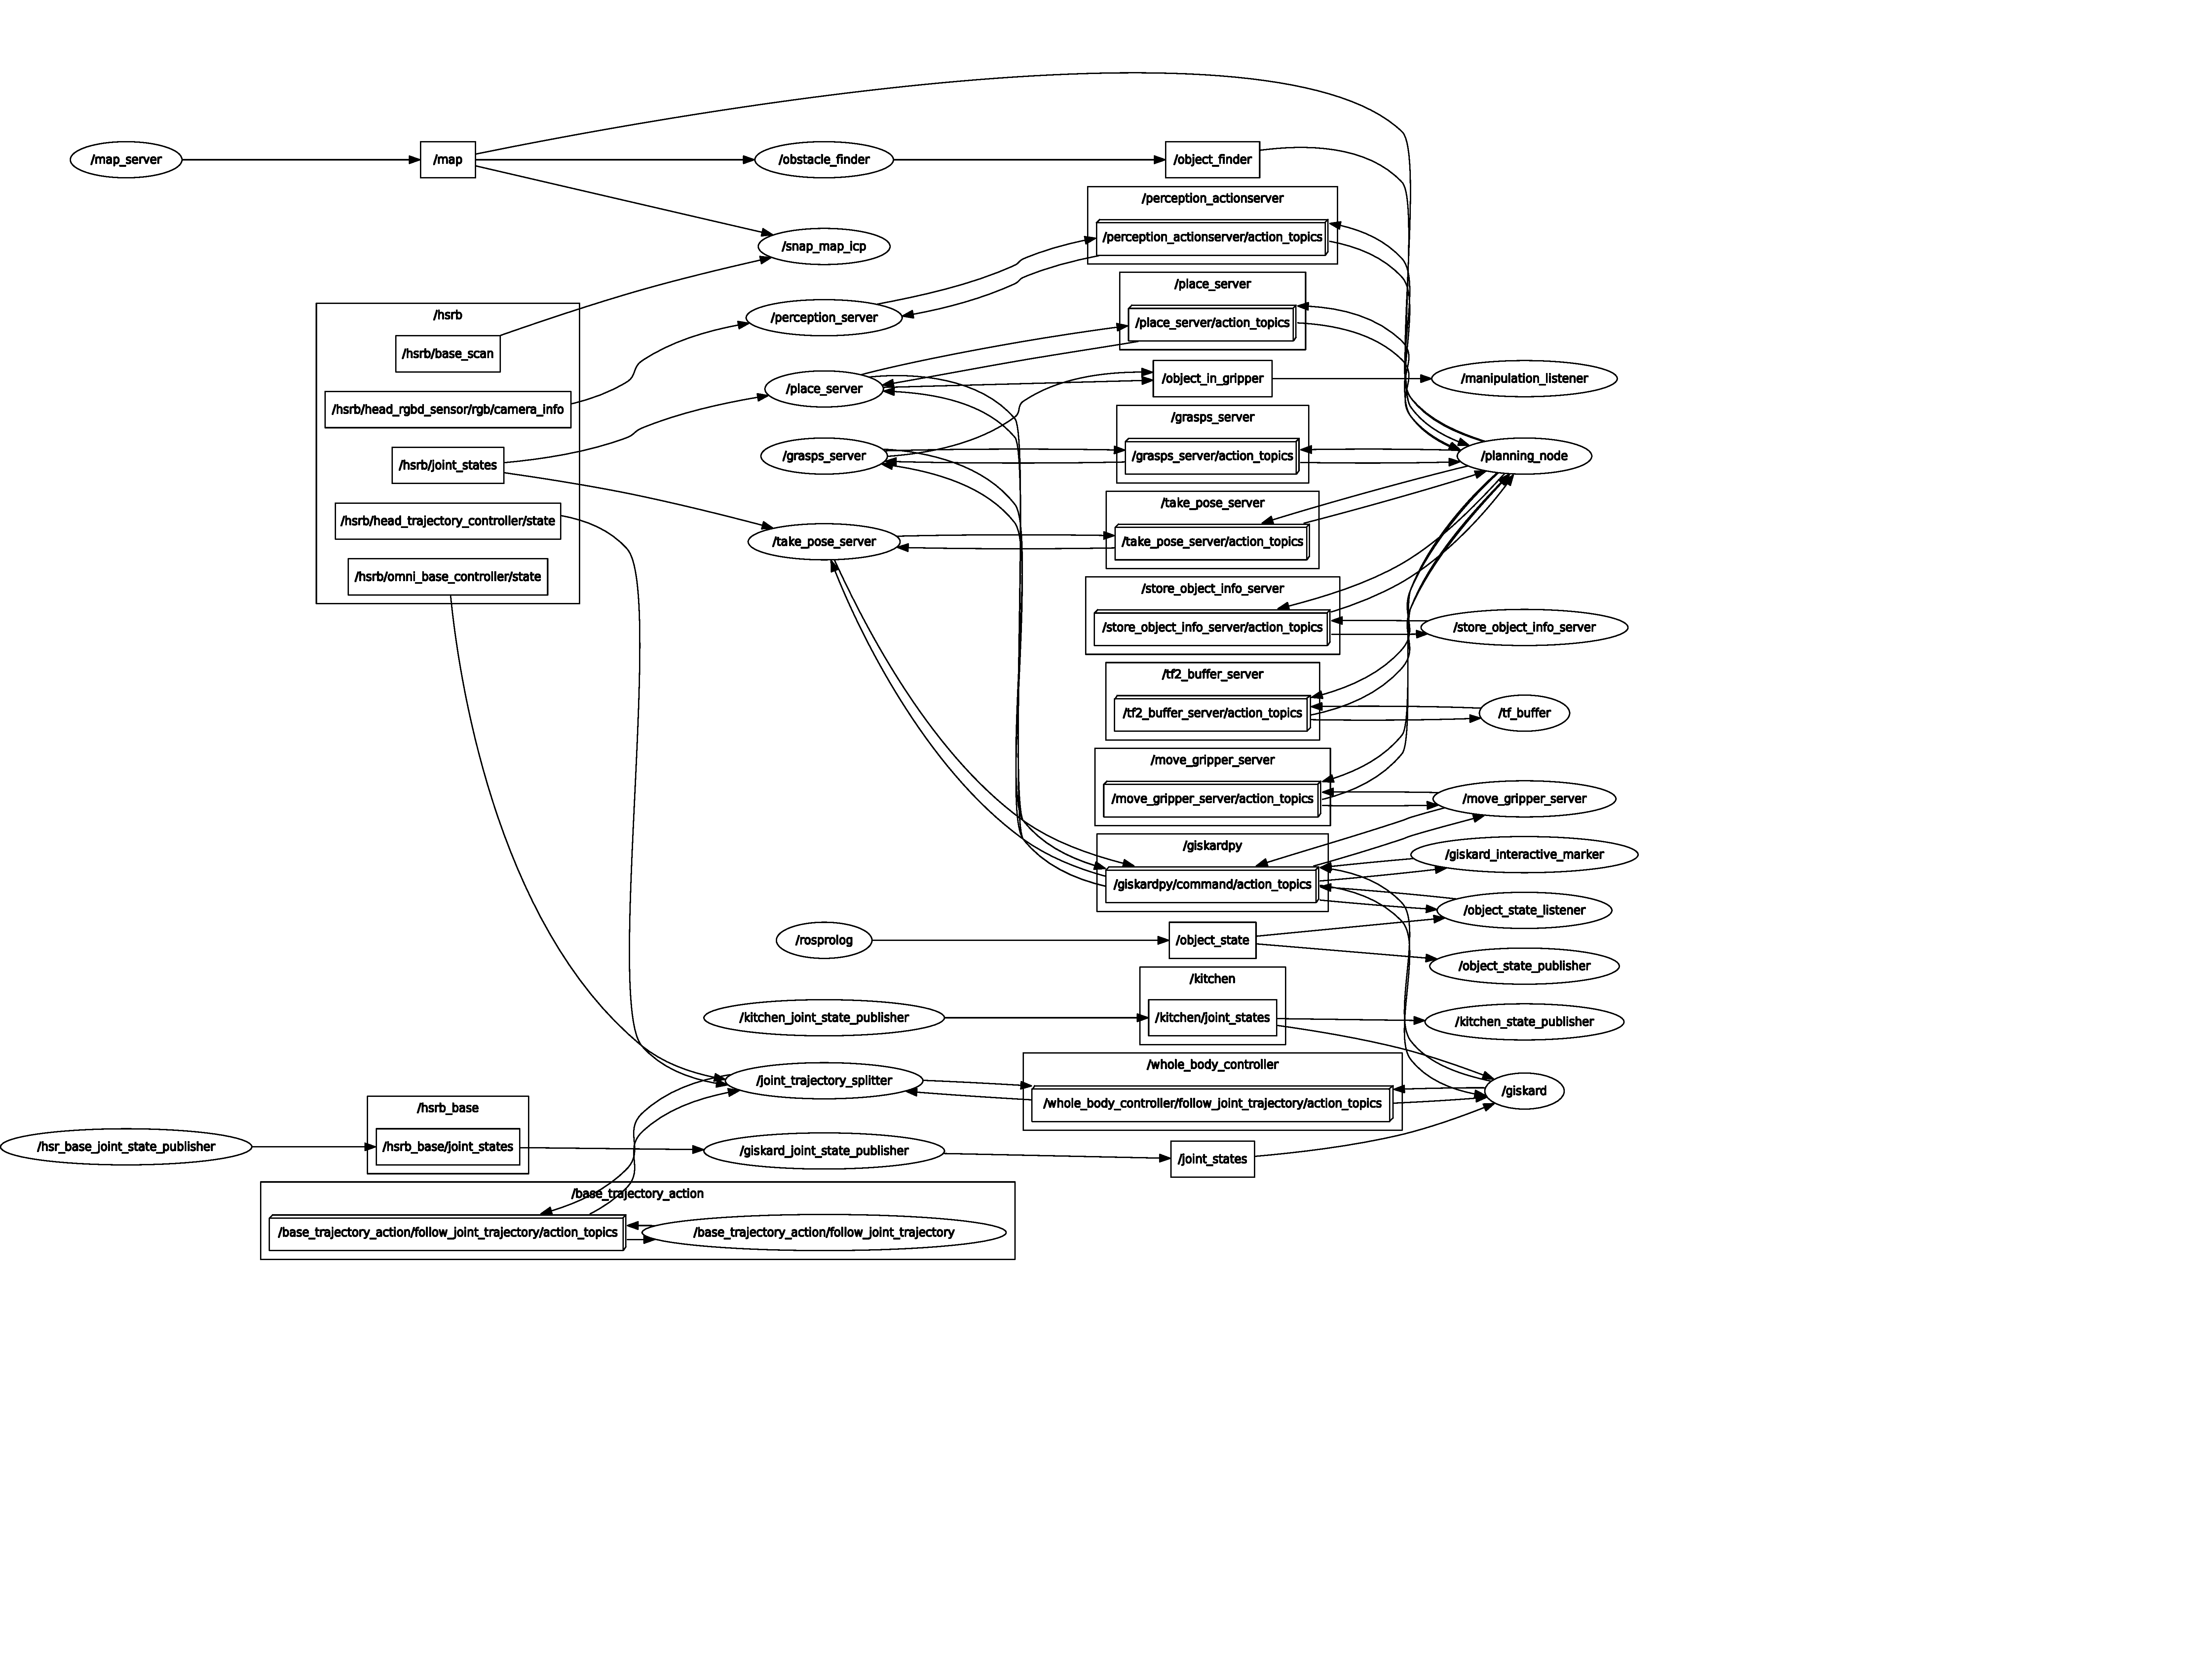
\includegraphics[width=1.5\textwidth]{pictures/diagramms/rqt_interfaces_cleanup_vertical}
			\caption{rqt\_graph during the execution of Clean Up}
			\label{cleanup-interfaces}
		\end{figure}
		\endgroup
\end{document}